\noindent\begin{minipage}{7cm}
\begin{description}
\item[Objectif :] aborder les notions d'algo\-rithme, d'algorithmique et de pro\-gram\-mation.
\end{description}
\end{minipage}
\mbox{}\hfill
\begin{tabular}{c}
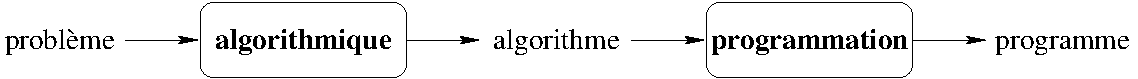
\includegraphics[width=8cm]{informatique-paysage.pdf}
\end{tabular}

%-------------------------------------------------------------------------
\subsection{Exemple}\label{ex:restaurant}
%-------------------------------------------------------------------------

\paragraph{Objectif :} 
Un touriste veut rejoindre le restaurant «~le bouche à oreille~»
à partir de son hôtel «~Kyriad~» (voir plan ci-dessous).

$$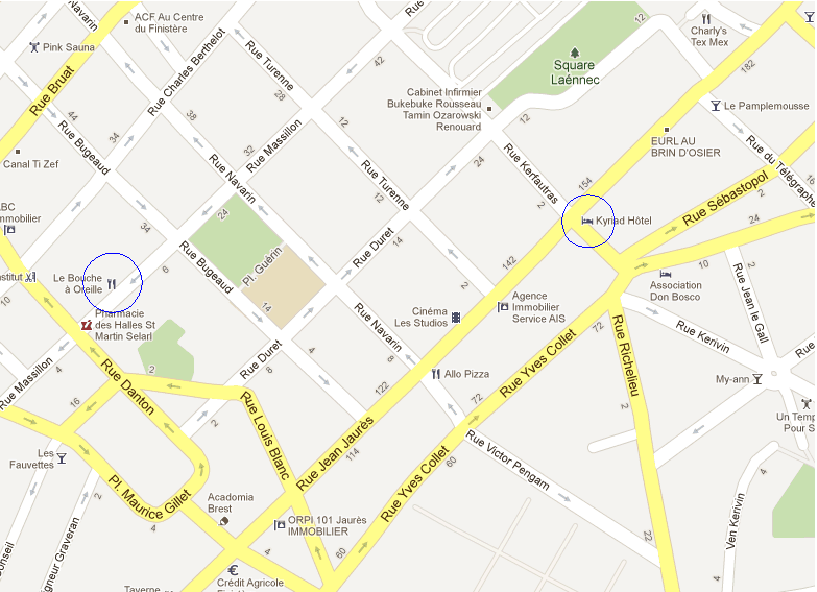
\includegraphics[width=0.9\textwidth]{plan.pdf}$$

\paragraph{Méthode :} 
Il s'agit ici de décrire une suite ordonnée d'instructions
(\emph{aller tout droit}, \emph{prenez la troisième à droite}\ldots)
qui manipulent des données (\emph{carrefours}, \emph{rues}\ldots)
pour réaliser la tâche désirée (\emph{aller au restaurant}).

\paragraph{Questions} 

\begin{question}[«~aller au restaurant~» : itinéraire] 
Proposer une suite d'instructions qui décrit un itinéraire pour aller
de l'hôtel au restaurant.
\end{question}

On doit toujours vérifier que la description proposée ne contient que des instructions compréhensibles par celui qui devra l'exécuter et qu'elle réalise bien exactement la tâche pour laquelle elle a été conçue.
\begin{question}[«~aller au restaurant~» : vérification]
Faire vérifier l'itinéraire proposé par une tier\-ce personne qui exécutera 
scrupuleusement les instructions dans l'ordre annoncé et vérifiera qu'elle
se rend bien de l'hôtel au restaurant. 
\end{question}

%-------------------------------------------------------------------------
\subsection{Généralisation}
%-------------------------------------------------------------------------
Un algorithme est une suite ordonnée d'instructions qui indique la démarche à suivre pour résoudre une série de problèmes équivalents. 

L'algorithmique est la science des algorithmes. Elle s'intéresse à l'art de construire des algorithmes ainsi qu'à caractériser leur validité, leur robustesse, leur réutilisabilité,
leur complexité et leur efficacité.

\begin{question}[algorithme : validité] 
La validité d'un algorithme est son aptitude à réaliser exactement la tâche
pour laquelle il a été conçu.\\
L'itinéraire «~aller au restaurant~» proposé est-il valide ?
\end{question}

\begin{question}[algorithme : robustesse] 
La robustesse d'un algorithme est son aptitude à se protéger de conditions 
anormales d'utilisation.\\
L'itinéraire «~aller au restaurant~» proposé s'applique-t-il aussi bien à une voiture qu'à un piéton ?
L'itinéraire est-il «~robuste~» ?
\end{question}

\begin{question}[algorithme : réutilisabilité] 
La réutilisabilité d'un algorithme est son aptitude à être réutilisé pour résoudre
des tâches équivalentes à celle pour laquelle il a été conçu.\\
L'itinéraire «~aller au restaurant~» proposé s'applique-t-il pour le restaurant «~Tex Mex~» du plan ?
L'itinéraire est-il «~réutilisable~» ?
\end{question}

\begin{question}[algorithme : complexité] 
La complexité d'un algorithme est le nombre d'instructions élémentaires à exécuter pour
réaliser la tâche pour laquelle il a été conçu.\\
Pour l'itinéraire «~aller au restaurant~» proposé, quelle pourrait être l'instruction élémentaire pour un piéton ?
\end{question}

\begin{question}[algorithme : efficacité] 
L'efficacité d'un algorithme est son aptitude à utiliser de manière optimale
les ressources du matériel qui l'exécute.\\
Dans l'itinéraire «~aller au restaurant~» proposé, n'existerait-il pas un raccourci 
piétonnier pour aller plus vite au restaurant ?
L'itinéraire est-il le plus «~efficace~» pour un piéton ? pour une «~voiture~» ?
\end{question}

L'algorithmique permet ainsi de passer d'un problème à résoudre à un algorithme
qui décrit la démarche de résolution du problème, en caractérisant l'algorithme retenu. 
La programmation a alors pour rôle de traduire cet
algorithme dans un langage «~compréhensible~» par l'ordinateur afin qu'il
puisse exécuter l'algorithme automatiquement.

%-------------------------------------------------------------------------
\subsection{Applications}
%-------------------------------------------------------------------------
\begin{question}[algorithme : tracés de polygones réguliers]
On cherche à faire dessiner une figure polygonale
sur la plage à quelqu'un qui a les yeux bandés.
Pour cela, on ne dispose que de 2 commandes orales :
avancer de $n$ pas en avant ($n$ est un nombre entier de pas) et 
tourner à gauche d'un angle $\theta$ (rotation sur place de $\theta$).
\begin{enumerate}
\item Faire dessiner un triangle équilatéral de 10 pas de côté.
\item Faire dessiner un carré de 10 pas de côté.
\item Faire dessiner un hexagone régulier de 10 pas de côté.
\item Faire dessiner un polygone régulier de $n$ côtés de 10 pas chacun.
\end{enumerate}
\end{question}

\begin{question}[algorithme : propriétés]
Quelle figure géométrique dessine-t-on en exécutant dans l'ordre la suite d'instructions 
ci-dessous ?
\begin{enumerate}
	\item avance de 2 pas,
	\item tourne à gauche de $90^\circ$,
	\item avance de 3 pas,
	\item tourne à gauche de $90^\circ$,
	\item avance de 4 pas,
	\item tourne à gauche de $90^\circ$,
	\item avance de 5 pas,
	\item tourne à gauche de $90^\circ$,
	\item avance de 6 pas.
\end{enumerate}
Discuter des propriétés de cet algorithme : validité, robustesse, réutilisabilité, complexité, efficacité.
\end{question}

%%-------------------------------------------------------------------------
%\subsection{QCM}
%%-------------------------------------------------------------------------
%\begin{enumerate}
%\item L'informatique est la science
%	\begin{enumerate}
%	\item des dispositifs dont le fonctionnement dépend de 
%		la circulation d'électrons
%	\item des signaux électriques porteurs d'information ou d'énergie
%	\item du traitement automatique de l'information
%	\item de la commande des appareils fonctionnant sans intervention humaine
%	\end{enumerate}
%\item Le logiciel est
%	\begin{enumerate}
%	\item la mémoire de l'ordinateur
%	\item l'ensemble de dispositifs physiques utilisés pour traiter
%		automatiquement des informations
%	\item l'ensemble des données manipulées par les instructions
%	\item un ensemble structuré d'instructions décrivant un traitement d'informations
%		à faire réaliser par un matériel informatique
%	\end{enumerate}
%\item L'algorithmique est la science
%	\begin{enumerate}
%	\item des algorithmes
%	\item des langages de programmation
%	\item des instructions
%	\item des données traitées par les algorithmes
%	\end{enumerate}
%\item Un algorithme est
%	\begin{enumerate}
%	\item un ensemble de programmes remplissant une fonction déterminée,
%		permettant l'accomplissement d'une tâche donnée
%	\item une suite ordonnée d'instructions qui indique la démarche 
%		à suivre pour résoudre une série de problèmes équivalents
%	\item le nombre d'instructions élémentaires à exécuter pour
%		réaliser une tâche donnée
%	\item un ensemble de dispositifs physiques utilisés pour traiter
%		automatiquement des informations
%	\end{enumerate}
%\item La validité d'un algorithme est son aptitude
%	\begin{enumerate}
%	\item à utiliser de manière optimale les ressources du matériel qui l'exécute
%	\item à être réutiliser pour résoudre des tâches équivalentes à celle pour 
%		laquelle il a été conçu
%	\item à se protéger de conditions anormales d'utilisation
%	\item à réaliser exactement la tâche pour laquelle il a été conçu
%	\end{enumerate}
%\item La complexité d'un algorithme est
%	\begin{enumerate}
%	\item le nombre de fois où l'algorithme est utilisé dans un programme
%	\item le nombre de données manipulées par les instructions de
%		l'algorithme
%	\item le nombre d'octets occupés en mémoire par l'algorithme
%	\item le nombre d'instructions élémentaires à exécuter pour
%		réaliser la tâche pour laquelle il a été conçu
%	\end{enumerate}
%\end{enumerate}

%-------------------------------------------------------------------------
%\newpage
\subsection{Entraînement}
%-------------------------------------------------------------------------

%-------------------------------------------------------------------------
\subsubsection{Enoncé}
%-------------------------------------------------------------------------
\paragraph{Contexte :} «~Les cerveaux des Shadoks avaient une capacité tout à fait limitée.
Ils ne comportaient en tout que 4 cases. 
Comme ils n'avaient que 4 cases, évidemment les Shadoks ne connaissaient
pas plus de 4 mots :  \textsc{ga, bu, zo et meu}. 
Etant donné qu'avec 4 mots, ils ne pouvaient pas compter plus loin que 4, 
le Professeur Shadoko avait réformé tout ça : 
\begin{itemize} 
\item Quand il n'y a pas de Shadok, on dit \ga{} et on écrit \ga{}. 
\item Quand il y a un Shadok de plus, on dit \bu{} et on écrit \bu{}. 
\item Quand il y a encore un Shadok, on dit \zo{} et on écrit \zo{}. 
\item Et quand il y en a encore un autre, on dit \meu{} et on écrit \meu{}. 
\end{itemize} 
Tout le monde applaudissait très fort et trouvait ça génial sauf le Devin Plombier 
qui disait qu'on n'avait pas idée d'inculquer à des enfants des bétises pareilles 
et que Shadoko, il fallait le condamner. 
Il fut très applaudi aussi. Les mathématiques, 
cela les intéressait, bien sûr, mais brûler le professeur, c'était intéressant aussi, 
faut dire. 
Il fut décidé à l'unanimité qu'on le laisserait parler et qu'on le brûlerait après, 
à la récréation.
\begin{itemize}
\item Répétez avec moi : \meu{} \zo{} \bu{} \ga{}\ldots{} \ga{} \bu{} \zo{} \meu{}. 
\item Et après! ricanait le Plombier. 
\item Si je mets un Shadok en plus, évidemment, je n'ai plus assez 
de mots pour les compter, alors c'est très simple : on les jette dans une poubelle, 
et je dis que j'ai \bu{} poubelle. 
Et pour ne pas confondre avec le \bu{} du début, 
je dis qu'il n'y a pas de Shadok à côté de la poubelle et j'écris \bu{} \ga{}. 
\bu{} Shadok à côté de la poubelle: \bu{} \bu{}. Un autre : \bu{}  \zo{}. Encore un autre : \bu{} \meu{}. 
On continue. \zo{} poubelles et pas de Shadok à côté : \zo{} \ga{}\ldots{} 
\meu{} poubelles et \meu{} Shadoks à côté : \meu{} \meu{}. 
Arrivé là, si je mets un Shadok en plus, il me faut une autre poubelle. 
Mais comme je n'ai plus de mots pour compter les poubelles, je m'en débarrasse 
en les jetant dans une grande poubelle. 

J'écris \bu{} grande poubelle avec pas de petite poubelle 
et pas de Shadok à côté: \bu{} \ga{} \ga{}, et on continue\ldots{} \bu{} \ga{} \bu{},
\bu{} \ga{} \zo{}\ldots{} \meu{} \meu{} \zo{},  \meu{} \meu{} \meu{}.
Quand on arrive là et qu'on a trop de grandes poubelles pour pouvoir les compter, 
eh bien, on les met dans une super-poubelle, on écrit \bu{} \ga{} \ga{} \ga{}, 
et on continue\ldots{}~»
\end{itemize}
\mbox{}\hfill\bsc{Jacques Roussel}, \emph{Les Shadoks : \ga{} \bu{} \zo{} \meu{}},
Circonflexe, 2000.

\paragraph{Remarque préliminaire:} Le calcul «~Shadok~» repose sur les 4 chiffres \ga, \bu, \zo{} et \meu{} qui peuvent \^etre assimilés aux 4 chiffres 0, 1, 2 et 3 : 
\begin{itemize} 
\item «~Quand il n'y a pas de Shadok, on dit \ga{} et on écrit \ga{}.~» \hfill$\Rightarrow \ga{} = 0$
\item «~Quand il y a un Shadok de plus, on dit \bu{} et on écrit \bu{}.~» 
\hfill$\Rightarrow \bu{} = 1$
\item «~Quand il y a encore un Shadok, on dit \zo{} et on écrit \zo{}.~» 
\hfill$\Rightarrow \zo{} = 2$
\item «~Et quand il y en a encore un autre, on dit \meu{} et on écrit \meu{}.~» 
\hfill$\Rightarrow \meu{} = 3$
\end{itemize} 
Il s'agit donc d'une \textbf{numération en base 4}.

Les différentes «~poubelles Shadok~» correspondent respectivement
aux 4-aines (les «~dizaines~~» de la base 4 : $4^1$), 
aux 16-aines (les «~centaines~» de la base 4 : $4^2$), 
aux 64-aines (les «~~milliers~» de la base 4 : $4^3$) :
\begin{itemize}
\item «~Si je mets un Shadok en plus, évidemment, je n'ai plus assez 
de mots pour les compter, alors c'est très simple : on les jette dans une poubelle, 
et je dis que j'ai \bu{} poubelle. 
Et pour ne pas confondre avec le \bu{} du début, 
je dis qu'il n'y a pas de Shadok à côté de la poubelle et j'écris \bu{} \ga{}. 
\bu{} Shadok à côté de la poubelle: \bu{} \bu{}. Un autre : \bu{}  \zo{}. Encore un autre : \bu{} \meu{}. 
On continue. \zo{} poubelles et pas de Shadok à côté : \zo{} \ga{}\ldots{} 
\meu{} poubelles et \meu{} Shadoks à côté : \meu{} \meu{}. 
Arrivé là, si je mets un Shadok en plus, il me faut une autre poubelle. 
Mais comme je n'ai plus de mots pour compter les poubelles, je m'en débarrasse 
en les jetant dans une grande poubelle. 

J'écris \bu{} grande poubelle avec pas de petite poubelle 
et pas de Shadok à côté: \bu{} \ga{} \ga{}, et on continue\ldots{}~»
\end{itemize}
Il s'agit donc d'un \textbf{système de notation positionnelle} identique
à celui qu'on utilise tous les jours. On peut donc «~poser~» 
les calculs comme en base décimale.

\paragraph{Rappel:} Un entier positif en base $b$ est représenté par une suite de
	chiffres {$(r_nr_{n-1}\ldots r_1r_0)_b$}
	où les $r_i$ sont des chiffres de la base $b$ ($0\leq r_i < b$).
	Ce nombre a pour valeur:
	$${r_nb^n + r_{n-1}b^{n-1} + \ldots + r_1b^1 + r_0b^0 = 
        \sum^{i=n}_{i = 0} r_ib^i}$$

\paragraph{Objectif :} exécuter les algorithmes de calcul arithmétique ($+$, $-$, $\times$, $\div$)
dans une base non décimale, ici la base «~Shadok~».

\paragraph{Méthode :} poser les opérations en base $b$.

\paragraph{Vérification :} vérifier les calculs d'une part
en passant par la base 10 et d'autre part, en effectuant la preuve par $b-1$ 
(preuve par 3 en base 4, preuve par 9 en base 10).

%-------------------------------------------------------------------------
\subsubsection{Exemples}
%-------------------------------------------------------------------------
\begin{enumerate}
\item Soit à additionner $x = $ \bu{} \bu{} \ga{} \meu{} et $y = $ \zo{} \bu{} \zo{} \zo{}. 
Compte-tenu du système de notation positionnelle en base 4 :  $x = (1103)_4 = 1\cdot4^3 + 1\cdot4^2 + 0\cdot4^1 + 3\cdot4^0 = (83)_{10}$ 
et $y = (2122)_4 = 2\cdot4^3 + 1\cdot4^2 + 2\cdot4^1 + 2\cdot4^0 = (154)_{10}$.

On pose donc l'opération en base 4, puis on vérifie en base 10.

	{\footnotesize
	$$\begin{tabular}{|c|c|}
	\hline
	\makebox[4cm]{\textbf{calcul direct}} & \makebox[4cm]{\textbf{vérification}} \\
	en base 4 & en base 10 \\
	\hline
	\begin{tabular}{rrrrr}
	    & 1 & 1 & $^1$0 & 3 \\
	$+$ & 2 & 1 &     2 & 2 \\
	\hline
	$=$ & 3 & 2 & 3 & 1 
	\end{tabular} 
	& 
	\begin{tabular}{rrrr}
	    &   & 8 & 3 \\
	$+$ & $^1$1 & 5 & 4 \\
	\hline
	$=$ & 2 & 3 & 7 
	\end{tabular}\\
	\hline
	\multicolumn{2}{c}{}\\[-2mm]
	\multicolumn{2}{c}{$z=x+y = (3231)_4 = 3\cdot4^3 + 2\cdot4^2 + 3\cdot4^1 + 1\cdot4^0 = (237)_{10}$}  
	\end{tabular}$$}  
	
En plus de la vérification par le passage en base 10, on peut effectuer les «~preuves~»
par $b-1$ : «~preuve~» par 9 en base 10 (où 9 «~vaut~» 0), «~preuve~» par 3 en base 4 (où 3 «~~vaut~~» 0). Rappelons que si
la preuve par $b-1$ échoue, le résultat de l'opération est faux; par contre, si la preuve 
par $b-1$ réussit, le résultat de l'opération n'est pas forcément exact (2 erreurs peuvent se compenser). 
	
	{\scriptsize
	$$\begin{tabular}{|c|c|}
	\hline
		\makebox[4cm]{\textbf{preuve par 3}} & \makebox[4cm]{\textbf{preuve par 9}} \\
		en base 4 & en base 10 \\
	\hline
		\begin{tabular}{c|c|c}
		& $x=\mathbf{1103}$ & \\
		& \tiny $1+1+0+3 = 11$ & \\
		& \tiny $1 + 1 = 2$ & \\
		& \textbf{2} & \\
		\hline
		$z=\mathbf{3231}$  & \multirow{4}{0.5cm}{\huge$+$} & $\mathbf{2+1}$\\
		\tiny $3+2+3+1 = 21$ &                               & \tiny\\
		\tiny $2+1 = 3$      &                               & \tiny $2+1 = 3$\\
		\textbf{3}                 &                               & \textbf{3} \\
		\hline
		& $y=\mathbf{2122}$ & \\
		& \tiny $2+1+2+2 = 13$ & \\
		& \tiny $1+3=10$ & \\
		& \tiny $1+0=1$ & \\
		& \textbf{1} & 
		\end{tabular} 
	& 
		\begin{tabular}{c|c|c}
		& $x=\mathbf{83}$ & \\
		& \tiny $8 + 3 = 11$ & \\
		& \tiny $1 + 1 = 2$ & \\
		& \textbf{2} & \\
		\hline
		$z=\mathbf{237}$ & \multirow{4}{0.5cm}{\huge$+$} & $\mathbf{2+1}$\\
		\tiny $2+3+7=12$ & & \\
		\tiny $1+2 = 3$ & & \tiny $2+1 = 3$\\
		\textbf{3} & & \textbf{3} \\
		\hline
		& $y=\mathbf{154}$ & \\
		& \tiny $1+5+4 = 10$ & \\
		& \tiny $1+0=1$ & \\
		& & \\
		& \textbf{1} & 
		\end{tabular}\\
	\hline
	\end{tabular}$$}  
	
Le passage par la base 10 et les «~preuves~» par 3 en base 4 et par 9 en base 10 
confirment le résultat obtenu par le calcul direct.
On obtient donc $(1103)_4 + (2122)_4 = (3231)_4$, soit en notation «~Shadok~» :\\
\bu{} \bu{} \ga{} \meu{} $+$ \zo{} \bu{} \zo{} \zo{} $=$ \meu{} \zo{} \meu{} \bu{}  


\item On opère à l'identique pour la soustraction des deux nombres
$x = $ \zo{} \zo{} \bu{} \zo{} et $y = $ \bu{} \zo{} \ga{} \bu{}.
	
	{\footnotesize
	$$\begin{tabular}{|c|c|}
	\hline
	\makebox[4cm]{\textbf{calcul direct}} & \makebox[4cm]{\textbf{vérification}} \\
	en base 4 & en base 10 \\
	\hline
	\begin{tabular}{rrrrr}
	    & 2 & 2 & 1 & 2 \\
	$-$ & 1 & 2 & 0 & 1 \\
	\hline
	$=$ & 1 & 0 & 1 & 1 
	\end{tabular} 
	& 
	\begin{tabular}{rrrr}
	    &    1 & $^1$6 & $^1$6 \\
	$-$ & $_1$ & $_1$9 &     7 \\
	\hline
	$=$ &   & 6 & 9 \\
	\end{tabular}\\
	\hline
	\multicolumn{2}{c}{}\\[-2mm]
	\multicolumn{2}{c}{$z=x-y = (1011)_4 = 1\cdot4^3 + 0\cdot4^2 + 1\cdot4^1 + 1\cdot4^0 = (69)_{10}$}	
	\end{tabular}$$}  

Pour les «~preuves~» par $b-1$, on considère l'addition $z+y = x$.
	{\scriptsize
	$$\begin{tabular}{|c|c|}
	\hline
		\makebox[4cm]{\textbf{preuve par 3}} & \makebox[4cm]{\textbf{preuve par 9}} \\
		en base 4 & en base 10 \\
	\hline
		\begin{tabular}{c|c|c}
		& $z=\mathbf{1011}$ & \\
		& \tiny  & \\
		& \tiny $1+0+1+1 = 3$ & \\
		& \textbf{3} & \\
		\hline
		$x=\mathbf{2212}$  	& \multirow{4}{0.5cm}{\huge$-$} & $\mathbf{3+1}$\\
		\tiny $2+2+1+2=13$  	&                               & \tiny $3+1=10$\\
		\tiny $1 + 3 = 10$  	&                               & \tiny $1+0=1$\\
		\textbf{1}                 	&                               & \textbf{1} \\
		\hline
		& $y=\mathbf{1201}$ & \\
		& \tiny $1+2+0+1 = 10$ & \\
		& \tiny $1+0=1$ & \\
		& \textbf{1} & 
		\end{tabular} 
	& 
		\begin{tabular}{c|c|c}
		& $z=\mathbf{69}$ & \\
		& \tiny $6+9=15$ & \\
		& \tiny $1+5=6$ & \\
		& \textbf{6} & \\
		\hline
		$x=\mathbf{166}$ & \multirow{4}{0.5cm}{\huge$-$} & $\mathbf{6+7}$\\
		\tiny $1+6+6=13$ & & \tiny $6+7 = 13$\\
		\tiny $1 + 3 = 4$ & & \tiny $1+3=4$\\
		\textbf{4} & & \textbf{4} \\
		\hline
		& $y=\mathbf{97}$ & \\
		& \tiny $9+7=16$ & \\
		& \tiny $1+6=7$ & \\
		& \textbf{7} & 
		\end{tabular}\\
	\hline
	\end{tabular}$$}  

Le passage par la base 10 et les «~preuves~» par 3 en base 4 et par 9 en base 10 
confirment le résultat obtenu par le calcul direct.
On obtient ainsi $(2212)_4 - (1201)_4 = (1011)_4$, soit en notation «~Shadok~» :\\
\zo{} \zo{} \bu{} \zo{} $-$ \bu{} \zo{} \ga{} \bu{} $=$ \bu{} \ga{} \bu{} \bu{} 

\item La procédure reste la même pour le multiplication des deux nombres
$x = $ \zo{} \bu{} \bu{} \zo{} et $y = $ \meu{} \bu{} \ga{}.

	{\footnotesize
	$$\begin{tabular}{|c|c|}
	\hline
	\makebox[6cm]{\textbf{calcul direct}} & \makebox[6cm]{\textbf{vérification}} \\
	en base 4 & en base 10 \\
	\hline
	\begin{tabular}{rrrrrrrr}
	         &   &   &   & 2 & 1 & 1 & 2 \\
	$\times$ &   &   &   &   & 3 & 1 & 0 \\
	\hline
	         &   &   &   & 0 & 0 & 0 & 0 \\
	$+$      &   &   & 2 & 1 & 1 & 2 &   \\
	$+$      & 1 & 3 & 0 & 0 & 2 &   &  \\
	\hline
	$=$      & 1 & 3 & 2 & 1 & 3 & 2 & 0 
	\end{tabular} 
	& 
	\begin{tabular}{rrrrr}
	        &  & 1 & 5 & 0 \\
	$\times$&  &   & 5 & 2 \\
	\hline
	        &   & 3 & 0 & 0 \\
	$+$     & 7 & 5 & 0 &   \\
	\hline
	$=$     & 7 & 8 & 0 & 0
	\end{tabular}    \\
	\hline
	\multicolumn{2}{c}{}\\[-2mm]
	\multicolumn{2}{c}{$z=x\times y = (1321320)_4 = 1\cdot4^6 + 3\cdot4^5 + 2\cdot4^4 + 1\cdot4^3 + 3\cdot4^2 + 2\cdot4^1 + 0\cdot4^0 = (7800)_{10}$}  
	\end{tabular}$$} 


	{\scriptsize
	$$\begin{tabular}{|c|c|}
	\hline
		\makebox[4cm]{\textbf{preuve par 3}} & \makebox[4cm]{\textbf{preuve par 9}} \\
		en base 4 & en base 10 \\
	\hline
		\begin{tabular}{c|c|c}
		& $x=\mathbf{2112}$ & \\
		& \tiny $2+1+1+2=12$ & \\
		& \tiny $1+2 = 3$ & \\
		& \textbf{3} & \\
		\hline
		$z=\mathbf{1321320}$ & \multirow{4}{0.5cm}{\huge$\times$}& $\mathbf{3\times1}$\\
		\tiny $1+3+2+1+3+2+0=30$  	&                               	& \tiny $3\times1=3$\\
		\tiny $3+0=3$  				&                               	& \tiny \\
		\textbf{3}                 	&                               	& \textbf{3} \\
		\hline	
		& $y=\mathbf{310}$ & \\
		& \tiny $3+1+0=10$ & \\
		& \tiny $1+0=1$ & \\
		& \textbf{1} & 
		\end{tabular} 
	& 
		\begin{tabular}{c|c|c}
		& $x=\mathbf{150}$ & \\
		& \tiny & \\
		& \tiny $1+5+0=6$ & \\
		& \textbf{6} & \\
		\hline
		$z=\mathbf{7800}$ & \multirow{4}{0.5cm}{\huge$\times$} & $\mathbf{6\times7}$\\
		\tiny $7+8+0+0=15$ & & \tiny $6\times7=42$\\
		\tiny $1 + 5 = 6$ & & \tiny $4+2=6$\\
		\textbf{6} & & \textbf{6} \\
		\hline
		& $y=\mathbf{52}$ & \\
		& \tiny  & \\
		& \tiny $5+2=7$ & \\
		& \textbf{7} & 
		\end{tabular}\\
	\hline
	\end{tabular}$$}  

Le passage par la base 10 et les «~preuves~» par 3 en base 4 et par 9 en base 10 
confirment le résultat obtenu par le calcul direct.
On a donc $(2112)_4 \times (310)_4 = (1321320)_4$, et en notation «~Shadok~» :\\
\zo{} \bu{} \bu{} \zo{} $\times$ \meu{} \bu{} \ga{} $=$ 
\bu{} \meu{} \zo{} \bu{} \meu{} \zo{} \ga{}  

\item Enfin, pour la division entière des deux nombres
$x = $ \meu{} \zo{} \bu{} \bu{} et $y = $ \bu{} \meu{} \zo{}:

	{\footnotesize
	$$\begin{tabular}{|c|c|}
	\hline
	\makebox[6cm]{\textbf{calcul direct}} & \makebox[6cm]{\textbf{vérification}} \\
	en base 4 & en base 10 \\
	\hline
	\begin{tabular}{rrrrr|rrr}
	\multicolumn{8}{c}{}\\[-2mm]
	         & 3 & $^1$2 & $^1$1 & 1 & 1 & 3 & 2 \\
	\cline{6-8}
	$-$      & $_1$1 & $_1$3 & 2 &   &   & 1 & 3 \\
	\cline{1-4}
	$=$      & 1 & 2 & 3 & $^1$1 &   &   &   \\
	$-$      & 1 & 1 & $_1$2 & 2 &   &   &   \\
	\cline{1-5}
	$=$      & 0 & 1 & 0 & 3 &   &   &   \\
	\multicolumn{8}{c}{}\\[-2mm]
	\end{tabular} 
	& 
	\begin{tabular}{rrrr|rr}
	        & 2 & 2 & 9 & 3 & 0 \\
	\cline{5-6}
	$-$     & 2 & 1 & 0 &   & 7 \\
	\cline{1-4}
	$=$     & 0 & 1 & 9 &   &   \\
	\end{tabular}    \\
	\hline
	\multicolumn{2}{c}{}\\[-2mm]
	\multicolumn{2}{c}{$q=x\div y = (13)_4 = 1\cdot4^1 + 3\cdot4^0 = (7)_{10}$ et
	$r=x \% y = (103)_4 = 1\cdot4^2 + 0\cdot4^1 + 3\cdot4^0 = (19)_{10}$}\\
	\multicolumn{2}{c}{$x = (x\div y)\times y + (x\% y) = q\times y + r$}  
	\end{tabular}$$} 

Pour les «~preuves~» par $b-1$, on considère la multiplication et l'addition $q\times y + r = x$.

	{\scriptsize
	$$\begin{tabular}{|c|c|}
	\hline
		\makebox[4cm]{\textbf{preuve par 3}} & \makebox[4cm]{\textbf{preuve par 9}} \\
		en base 4 & en base 10 \\
	\hline
		\begin{tabular}{c|c|c}
		& $q=\mathbf{13}$ & $r=\mathbf{103}$\\
		& \tiny $1+3=10$  & \tiny $1+0+3=10$\\
		& \tiny $1+0=1$   & \tiny $1+0=1$\\
		& \textbf{1}      & \textbf{1}\\
		\hline
		$x=\mathbf{3211}$ & \multirow{4}{0.5cm}{\huge$\div$}& $\mathbf{1\times3+1}$\\
		\tiny $3+2+1+1=13$  	&                               	& \tiny $1\times3 + 1=10$\\
		\tiny $1+3=10$  				&                               	& \tiny $1+0=1$ \\
		\textbf{1}                 	&                               	& \textbf{1} \\
		\hline	
		& $y=\mathbf{132}$ & \\
		& \tiny $1+3+2=12$ & \\
		& \tiny $1+2=3$    & \\
		& \textbf{3}       & 
		\end{tabular} 
	& 
		\begin{tabular}{c|c|c}
		& $q=\mathbf{7}$ & $r=\mathbf{19}$\\
		& \tiny          & \tiny $1+9=10$\\
		& \tiny          & \tiny $1+0=1$\\
		& \textbf{7}     & \textbf{1}\\
		\hline
		$x=\mathbf{229}$ & \multirow{4}{0.5cm}{\huge$\div$} & $\mathbf{7\times3+1}$\\
		\tiny $2+2+9=13$ & & \tiny $7\times3+1=22$\\
		\tiny $1 + 3 = 4$ & & \tiny $2+2=4$\\
		\textbf{4} & & \textbf{4} \\
		\hline
		& $y=\mathbf{30}$ & \\
		& \tiny  & \\
		& \tiny $3+0=3$ & \\
		& \textbf{3} & 
		\end{tabular}\\
	\hline
	\end{tabular}$$}  

Le passage par la base 10 et les «~preuves~» par 3 en base 4 et par 9 en base 10 
confirment le résultat obtenu par le calcul direct.
On a finalement $(3211)_4 \div (132)_4 = (13)_4$, et en notation «~Shadok~» :\\
\meu{} \zo{} \bu{} \bu{} $\div$ \bu{} \meu{} \zo{} $=$
\bu{} \meu{} ou \\
\meu{} \zo{} \bu{} \bu{} $=$ \bu{} \meu{} \zo{} $\times$ \bu{} \meu{} +
\bu{} \ga{} \meu{}


\end{enumerate}



%-------------------------------------------------------------------------
%\newpage
\subsubsection{Questions}
%-------------------------------------------------------------------------

\noindent\begin{minipage}[t]{7cm}
\begin{enumerate}
\item \meu{} \zo{} \ga{} \bu{} 	$\div$ \meu{} \zo{} \zo{}
\item \zo{} \bu{} \zo{} \meu{} 	$\div$ \zo{} \ga{} \bu{} 
\item \zo{} \bu{} \bu{} \zo{} 	$\div$ \zo{} \bu{} \ga{}
\item \zo{} \meu{} \bu{} \zo{} 	$\div$ \bu{} \ga{} \meu{} 
\item \meu{} \ga{} \zo{} \meu{} $\div$ \meu{} \ga{} \zo{} 
\item \bu{} \zo{} \bu{} \zo{} 	$\div$ \bu{} \ga{} \zo{}
\item \bu{} \ga{} \zo{} \meu{} 	$\div$ \meu{} \zo{} \zo{}
\item \zo{} \meu{} \ga{} \zo{} 	$\div$ \bu{} \meu{} \zo{}
\item \bu{} \bu{} \zo{} \zo{} 	$\div$ \bu{} \ga{} \bu{}
\item \zo{} \zo{} \ga{} \meu{} 	$\div$ \bu{} \ga{} \ga{}
\item \zo{} \ga{} \zo{} \meu{} 	$\div$ \zo{} \ga{} \zo{}
\item \bu{} \zo{} \ga{} \bu{} 	$\div$ \bu{} \zo{} \zo{} 
\end{enumerate}
\end{minipage}
\hfill
\begin{minipage}[t]{7cm}
\begin{enumerate}\setcounter{enumi}{12}
\item \bu{} \meu{} \meu{} \ga{} $\div$ \bu{} \meu{} \ga{}
\item \bu{} \meu{} \bu{} \ga{} 	$\div$ \meu{} \zo{} \meu{}
\item \meu{} \zo{} \ga{} \bu{}	$\div$ \zo{} \bu{} \ga{}
\item \meu{} \ga{} \meu{} \bu{} $\div$ \bu{} \meu{} \ga{} 
\item \zo{} \bu{} \meu{} \meu{} $\div$ \bu{} \ga{} \bu{}
\item \zo{} \ga{} \meu{} \meu{} $\div$ \bu{} \zo{} \ga{} 
\item \bu{} \ga{} \zo{} \meu{}  $\div$ \bu{} \ga{} \zo{}
\item \meu{} \bu{} \bu{} \zo{}  $\div$ \meu{} \bu{} \ga{}
\item \bu{} \ga{} \meu{} \bu{}  $\div$ \bu{} \ga{} \ga{}
\item \zo{} \meu{} \meu{} \ga{} $\div$ \zo{} \meu{} \ga{}
\item \meu{} \zo{} \bu{} \meu{} $\div$ \zo{} \zo{} \zo{} 
\item \meu{} \meu{} \ga{} \zo{} $\div$ \zo{} \meu{} \meu{} 
\end{enumerate}
\end{minipage}

%-------------------------------------------------------------------------
\subsection{Révisions}
%-------------------------------------------------------------------------

$$\begin{tabular}{|ll@{ : }l|}
\hline
\textbf{Cours} & \cite{cours} & chapitre 1, section 1.1 \\
\textbf{TD}    & \cite{td}    & exercices 1.1 à 1.4, 1.19 à 1.28 \\
\hline
\end{tabular}$$
